\documentclass{beamer}
\usepackage[utf8]{inputenc}
\usepackage{textpos} 
\usepackage{graphicx} 
\usepackage{wrapfig}
\usepackage{tikz}
\usetikzlibrary{shapes.geometric,calc}
\usepackage{amsmath}
\usepackage{amssymb}
\usepackage[framemethod=TikZ]{mdframed}
\usepackage{caption} 
\usetheme{Boadilla}
\usecolortheme{default}
\usepackage{lmodern}
\usepackage{array}
\usepackage{pgfgantt} % Ensure you have this package
\usepackage{pgf-umlsd}
\usepackage{listings}


\title[Rapport Projet] 
{Présentation PFA: Reconnaissance Faciale dans un environnement contrôlé}

\subtitle{Conception, Modélisation et Développement.}

\author[HANFAOUI.K et KAFIF.I] 
{HANFAOUI Karim\inst{1} \and KAFIF. Imane\inst{2}}

\institute[EMSI] 
{
  \inst{1} EMSI, 3ème Année INFO G9 - \\
  Karim.Hanfaoui@emsi-edu.ma \\
  \inst{2} EMSI, 3ème Année INFO G9 - \\
  Imane.Kafif@emsi-edu.ma 
}

\date[MAR 2025] 
{EMSI Les Orangers, Mars 2025}



\AtBeginSection[]
{
  \begin{frame}
    \frametitle{Table of Contents}
    \tableofcontents[currentsection]
  \end{frame}
}

\begin{document}

\begin{frame}
    \titlepage
    \begin{textblock*}{2cm}(9cm, -7.7cm) 
        
\includegraphics[height=0.7cm]{logo} 
    \end{textblock*}
\end{frame}

\begin{frame}
\frametitle{Table of Contents}
\tableofcontents
\end{frame}

\section{Acronymes et Terminologie}
\begin{frame}{Acronymes et Terminologie}
    \textbf{ML} : Machine Learning \\
    \textbf{DL} : Deep Learning \\
    \textbf{PCA} : Principal Components Analysis \\
    \textbf{SVD} : Singular Value Decomposition \\
    \textbf{SVM} : support-vector Machine (Supervised training algorithm) \\
\end{frame}

\begin{frame}
    \frametitle{List of Figures}
    \listoffigures 
\end{frame}
\begin{frame}
\begin{abstract}

\emph{This project explores the design and implementation of a PCA-based facial recognition system tailored for controlled environments (uniform lighting, neutral background, and standardized facial poses). The primary objective is to develop a lightweight, interpretable, and efficient solution that addresses the traditional limitations of Eigenfaces—such as sensitivity to minor variations (e.g., facial expressions, accessories)—while maintaining real-time performance and compliance with ethical standards.
}

\end{abstract}
\end{frame}
\section{Problématique}
\begin{frame}{C'est quoi notre Problématique}
    \begin{block}{Problématique}
    Comment concevoir un système de détection et reconnaissance faciale, basé sur l'Analyse en Composantes Principales (PCA), capable d'identifier efficacement les individus dans un environnement contrôlé (éclairage uniforme, fond neutre), tout en garantissant un temps de traitement adapté à un suivi de présence en temps réel, et en surmontant les limites inhérentes aux Eigenfaces face aux variations mineures (expressions faciales, accessoires) et aux contraintes de données réduites ?
    \end{block}
\end{frame}

\section{Hypothese}
\begin{frame}{Les hypotheses mises à respecter}
    \begin{block}{Hypothese}
    \item \textbf{Données d'entrée} : Les images sources ont une résolution minimale de 128×128 pixels et contiennent au moins un visage humain identifiable.
        \item \textbf{Ressources} : Les temps de traitement par image resteront inférieurs à 2 secondes sur du matériel grand public (CPU standard).
        \item \textbf{Évolutivité} : La chaîne de prétraitement peut gérer des lots de 100+ images sans dégradation significative des performances.\\
    \end{block}
\end{frame}

\section{Fonctionnalité Principale du Programme}
\begin{frame}{Fonctionnalité Principale du Programme}
    \begin{itemize}
        \item \textbf{Prétraitement des Images} : \textit{Préparation de dataset}.
        \begin{itemize}
            \item Détection et rognages des visages
            \item Conversion en gris (0-255)
            \item Alignement des visages
            \item Réduction du bruit (Application des filtres gaussiens ou médians)
        \end{itemize}

        \vspace{0.2cm}
        \begin{figure}[ht]
            \centering
            \scalebox{1}{%
                \begin{tabular}{*{7}{c}}
                    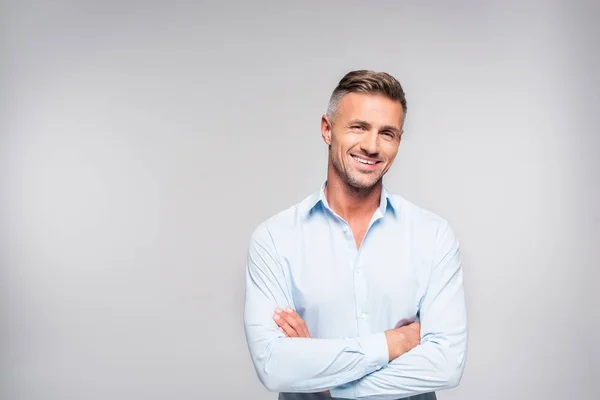
\includegraphics[height=1.2cm,keepaspectratio]{face_crop.jpg} & 
                    \raisebox{0.5cm}{$\Rightarrow$} & 
                    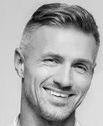
\includegraphics[height=1.2cm,keepaspectratio]{grayscale.jpg} & 
                    \raisebox{0.5cm}{$\Rightarrow$} & 
                    \includegraphics[height=1.2cm,keepaspectratio]{alignment.jpg} & 
                    \raisebox{0.5cm}{$\Rightarrow$} & 
                    \includegraphics[height=1.2cm,keepaspectratio]{denoise.jpg} \\
                    \scriptsize\textbf{(1) Détection} & & 
                    \scriptsize\textbf{(2) Conversion} & & 
                    \scriptsize\textbf{(3) Alignement} & & 
                    \scriptsize\textbf{(4) Débruitage} \\
                \end{tabular}%
            }
            \caption{Processus de prétraitement des images faciales}
            \label{fig:preprocessing_flow}
        \end{figure}
    \end{itemize}
\end{frame}

\begin{frame}{Fonctionnalité Principale du Programme}
    \begin{itemize}
        \item \textbf{Extraction des données avec ACP} : \textit{Préparation de dataset}.
        \begin{itemize}
            \item Calcul des EigenFaces (les vecteurs propres en relation.)
            \item Rédcuction de dimensions (sélection des composantes principales)
            \item Optimisation de nombre de composantes
        \end{itemize}
    \end{itemize}
\end{frame}

\begin{frame}{Conformité RGPD et Sécurité des Données}
    \begin{itemize}
        \item \textbf{Protection et gestion sécurisée des données faciales} :
        \begin{itemize}
            \item Conformité aux exigences du RGPD pour la collecte et le traitement des données personnelles.
            \item \textbf{Chiffrement des données sensibles} : Utilisation de l'algorithme AES-256 pour assurer la confidentialité et l'intégrité des données stockées.
            \item Mise en œuvre d’un accès restreint et d’une journalisation des accès afin d’assurer la traçabilité.
        \end{itemize}
        
    \end{itemize}
\end{frame}

\section{Comparaison FaceID vs. Notre Système}
\begin{frame}{FaceID vs. Notre Système}
\begin{center}
\begin{tabular}{|p{3cm}|p{4cm}|p{4cm}|}
\hline
\textbf{Critère} & \textbf{FaceID (Apple)} & \textbf{Notre Système (ACP+SVM)} \\
\hline
Acquisition & TrueDepth (IR 3D) & Images 2D prétraitées \\
\hline
Méthode & Deep learning + liveness & ACP (Eigenfaces) + SVM \\
\hline
Sécurité & Secure Enclave local & Chiffrement AES-256, accès restreint \\
\hline
Robustesse & Très robuste (variations) & Conditions contrôlées \\
\hline
RGPD & Traitement local & Conformité via chiffrement \\
\hline
Matériel & Matériel dédié (IR, projeteur) & Caméras standards \\
\hline
Performance & Déverrouillage instantané & Dépend de l'optimisation \\
\hline
\end{tabular}
\end{center}
\end{frame}

\begin{frame}{Estimation des Budgets}
    \begin{center}
    \begin{tabular}{|l|l|}
        \hline
        \textbf{Projet} & \textbf{Budget Estimé} \\
        \hline
        R\&D Apple Face ID & $\sim$1 milliard \$ (Not official) \\
        \hline
        Notre Projet & coffee+laptop+internet..:P \\
        \hline
    \end{tabular}
    \end{center}
    \vspace{0.5cm}
\end{frame}


\begin{frame}{Critères de Qualité d’un Logiciel}
    \begin{itemize}
        \item \textbf{Utilité} : Répondre précisément aux besoins.
        \item \textbf{Utilisabilité} : Facilité d'apprentissage et d'interaction.
        \item \textbf{Fiabilité} : Fonctionnement sans défaillance.
        \item \textbf{Interopérabilité} : Interaction avec d'autres systèmes.
        \item \textbf{Performance} : Rapidité et efficacité en gestion des ressources.
        \item \textbf{Portabilité} : Adaptabilité à différents environnements.
        \item \textbf{Réutilisabilité} : Réutilisation des composants.
        \item \textbf{Facilité de maintenance} : Correction et mise à jour aisées.
    \end{itemize}
\end{frame}

\section{Les Parties Prenantes}
\begin{frame}{Les Parties Prenantes}

    \begin{center}
    \begin{tabular}{|p{5cm}|p{6cm}|}
    \hline
    \textbf{Partie Prenante} & \textbf{Rôle/Responsabilités} \\
    \hline
    Équipe Technique & 
    \begin{itemize}
        \item Développeurs : Implémentation des algorithmes PCA
        \item Data Scientists : Optimisation des paramètres et validation
    \end{itemize} \\
    \hline
    Utilisateurs Finaux & 
    Employés/membres interagissant quotidiennement avec le système (pointage, accès sécurisé) \\
    \hline
    Responsables Sécurité & 
    Vérification du respect RGPD, gestion des risques liés aux données biométriques \\
    \hline
    Direction/Management & 
    Validation budgétaire, approbation du déploiement à l'échelle organisationnelle \\
    
    \hline
    \end{tabular}
\end{center}
    
\end{frame}

\begin{frame}{Les Parties Prenantes}
    \begin{center}
    \begin{tabular}{|p{5cm}|p{6cm}|}
    \hline
    Équipe Juridique & 
    Rédaction des clauses de consentement, conformité du stockage des données \\
    \hline
    Fournisseurs de Données & 
    Collecte et partage des photos de visages pour l'entraînement du modèle \\
    \hline
    Fournisseurs Matériels & 
    Intégration technique des caméras/GPUs et maintenance du matériel \\
    \hline
    Partenaires Académiques & 
    Collaboration sur l'optimisation mathématique des algorithmes PCA \\
    \hline
    \end{tabular}
\end{center}
    
\end{frame}

\section{Diagramme de GANTT}
\begin{frame}{Diagramme de GANTT}

    \def\mystartdate{2025-03-17}
    \def\myenddate{2025-04-04} % Shortened range for better fit
    

    \centering % Center the following content
    \scalebox{0.7}{ % Scale to fit inside Beamer slide
    \begin{ganttchart}[
        today={2025-03-28},
        today rule/.style={draw=red!80, dash pattern=on 3.5pt off 4.5pt, line width=1.5pt},
        today label font=\bfseries\small,
        today label=Today,
        hgrid style/.style={draw=black!70, line width=.1pt},
        vgrid={*1{draw=black!30, line width=.1pt}},
        x unit=0.8cm, % Reduce width per day
        inline,
        title height=1,
        y unit title=5mm,
        milestone inline label node/.style={right=2cm}, 
        bar inline label node/.style={right=2cm}, % Adjusted label padding
        bar label font=\mdseries\color{black!70},
        bar label node/.append style={right=-3cm},
        bar/.append style={draw=none, fill=blue!60}, 
        bar incomplete/.append style={fill=blue!30}, 
        bar progress label font=\mdseries\footnotesize\color{black!70},
        group/.append style={fill=blue!40}, 
        group label node/.append style={left=.4cm},
        link/.style={-latex, thick, ->, red, rounded corners=1mm},
        milestone/.append style={fill=red, rounded corners=1pt},
        time slot format=isodate
    ]{\mystartdate}{\myenddate}

    \gantttitlecalendar{week, weekday=letter, day} \\

    \ganttbar{Réunion 1}{2025-03-20}{2025-03-20} \\
    \ganttbar{Définition des fonctionnalité principales}{2025-03-20}{2025-03-22} \\
    \ganttbar{Réunion 2}{2025-03-21}{2025-03-21} \\
    \ganttbar{Recherche sur ACP}{2025-03-21}{2025-03-24} \\
    \ganttbar{Étude de faisabilité}{2025-03-23}{2025-03-26} \\
    \ganttbar{Étude comparatif}{2025-03-24}{2025-03-27} \\
    \ganttbar{Réunion 3}{2025-03-24}{2025-03-24} \\
    \ganttbar{Réunion 4}{2025-03-28}{2025-03-28} \\
    \ganttbar{Rédaction du rapport}{2025-03-20}{2025-03-29}
    \end{ganttchart}
    } % End of scalebox
\end{frame}

\begin{frame}{Détection des visages}
    \begin{itemize}
        \item \textbf{Objectif :}  
              Identifier et localiser automatiquement les zones d'une image contenant des visages humains.
        \item \textbf{Principe de base :}  
              Il s'agit d'un problème de classification binaire : pour chaque sous-région (ou fenêtre) de l'image, la décision est « visage » ou « non-visage ».
    \end{itemize}
    \begin{figure}[ht]
        \centering
        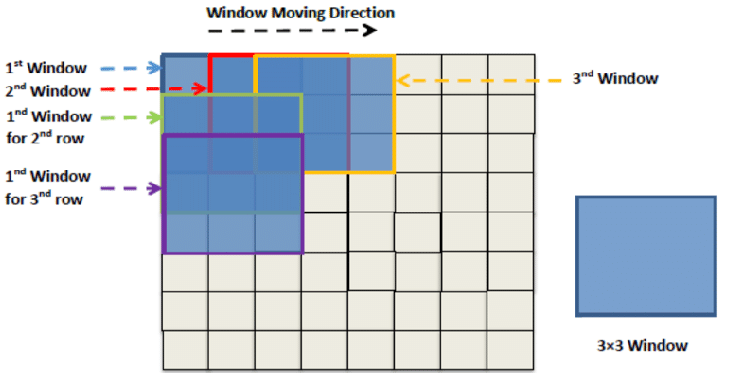
\includegraphics[width=0.6\textwidth]{sliding_window.png} % Remplacer par le nom de votre image
        \caption{Schéma illustrant la détection des visages par classification binaire}
        \label{fig:face_detection}
    \end{figure}
\end{frame}


\begin{frame}{Détection des visages}
    \begin{itemize}
        \item \textbf{Caractéristiques Haar :}  
              \begin{itemize}
                  \item Utilisation de caractéristiques simples (par exemple, la différence d'intensité entre deux zones rectangulaires adjacentes).
                  \item Ces caractéristiques permettent de capturer des motifs essentiels (ex : yeux foncés dans une zone claire).
              \end{itemize}
    \end{itemize}
    \begin{figure}[ht]
        \centering
        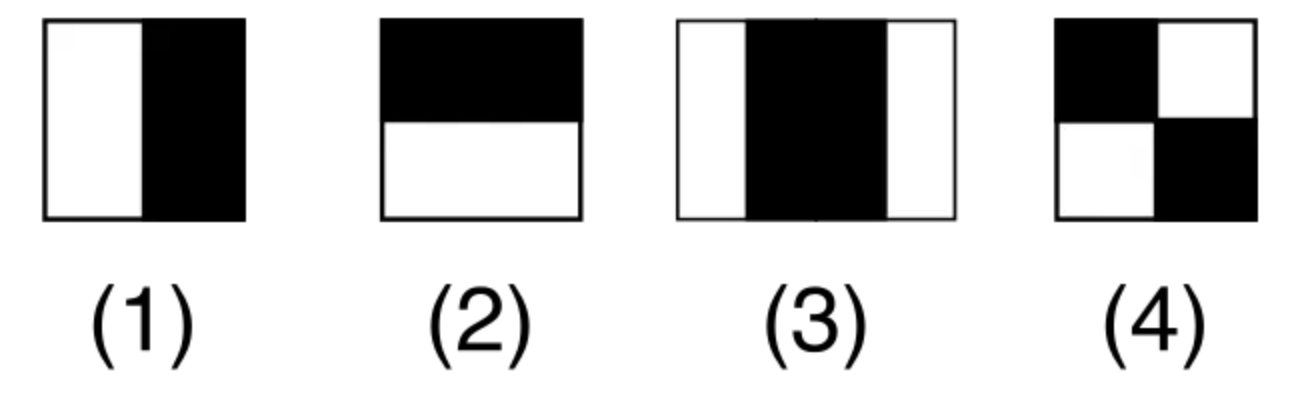
\includegraphics[width=0.6\textwidth]{haar_feature_1.png} % Remplacer par le nom de votre image
        \caption{Exemple de caractéristique Haar utilisée pour la détection de visages}
        \label{fig:haar_feature}
    \end{figure}
    
\end{frame}

\begin{frame}{Détection des visages}
    \begin{itemize}
        \item \textbf{Image intégrale :}  
              \begin{itemize}
                  \item Permet de calculer rapidement la somme des pixels dans n'importe quelle région rectangulaire.
                  \item Rend le calcul des caractéristiques Haar très efficace.
              \end{itemize}
    \end{itemize}
    \vspace{0.5cm}
    L'image intégrale \( II(x,y) \) d'une image \( I(x,y) \) est définie par :
    \[
        II(x,y) = \sum_{i=0}^{x} \sum_{j=0}^{y} I(i,j)
    \]
\end{frame}


\begin{frame}{Détection des visages}
    \begin{itemize}
        
        \item \textbf{La méthode Viola–Jones :}  
              \begin{itemize}
                  \item Combine un grand nombre de classificateurs faibles (basés sur les caractéristiques Haar) pour former un classificateur fort.
                  \item Utilise l'algorithme AdaBoost pour sélectionner et pondérer les caractéristiques les plus discriminantes.
                  \item Organise ces classificateurs sous forme d'une cascade : les premières étapes rejettent rapidement la majorité des sous-régions non pertinentes, seules les régions prometteuses passent aux étapes suivantes.
              \end{itemize}
    \end{itemize}
\end{frame}


\begin{frame}{Détection des visages}
    \begin{itemize}
        \item \textbf{Processus de détection :}
              \begin{enumerate}
                  \item \textbf{Prétraitement :} Convertir l'image en niveaux de gris.
                  \item \textbf{Calcul de l'image intégrale :} Facilite le calcul rapide des sommes sur des zones rectangulaires.
                  \item \textbf{Extraction de fenêtres :} Parcourir l'image avec une fenêtre glissante à différentes échelles.
                  \item \textbf{Calcul des caractéristiques :} Pour chaque fenêtre, calculer les valeurs des caractéristiques Haar.
                  \item \textbf{Classification binaire :} Appliquer la cascade de classificateurs pour décider si la fenêtre contient un visage.
              \end{enumerate}
    \end{itemize}
\end{frame}

\section{Petite Intro à l'ACP}
\begin{frame}{L'ACP, c'est quoi ?}
    \textbf{Analyse en Composantes Principales (ACP)} est une technique statistique utilisée pour :
    \begin{itemize}
        \item Réduire la dimensionnalité des données tout en conservant l'essentiel de l'information.
        \item Identifier les directions principales de variation des données.
        \item Faciliter la visualisation et l'interprétation des structures complexes.
    \end{itemize}
    
    \textbf{Principe :} Trouver des nouvelles variables (composantes principales) qui sont des combinaisons linéaires des variables d'origine et qui maximisent la variance.
    
    \textbf{Applications :}
    \begin{itemize}
        \item Compression et réduction de bruit.
        \item Visualisation de données en haute dimension.
        \item Prétraitement pour l'apprentissage automatique.
    \end{itemize}
    
\end{frame}

\begin{frame}{L'ACP, exemple:}
    \begin{itemize}
        \item \textbf{Compression des Images} : 
        \begin{itemize}
            \item Avantage: Réduction du bruit et la taille du fichier.
        \end{itemize}

        \vspace{0.2cm}
        \begin{figure}[ht]
            \centering
            \scalebox{1}{%
                \begin{tabular}{*{7}{c}}
                    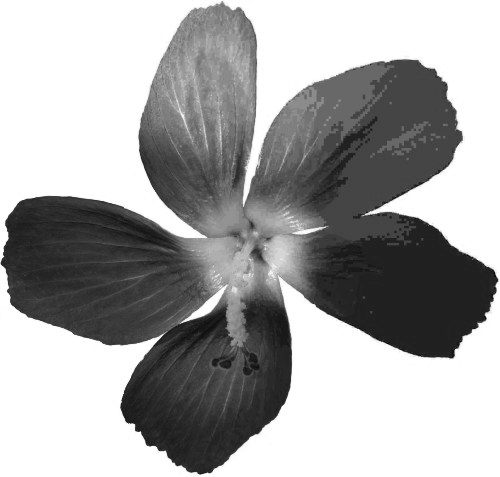
\includegraphics[height=4.5cm,keepaspectratio]{original_image.png} & 
                    \raisebox{2cm}{$\Rightarrow$} & 
                    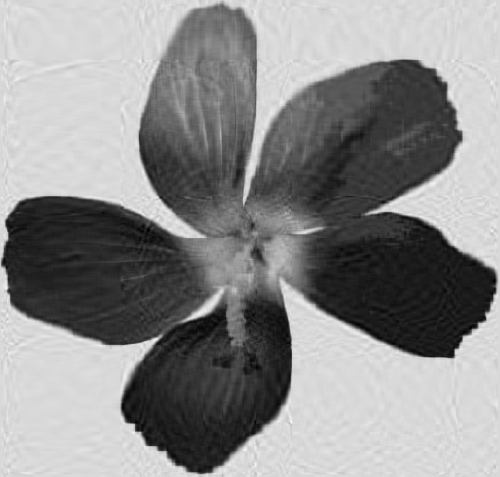
\includegraphics[height=5cm,keepaspectratio]{compressed_image.png} \\
                    \scriptsize\textbf{(1) Original} & & 
                    \scriptsize\textbf{(2) Réduite à 50 composantes} \\
                \end{tabular}%
            }
            \caption{Processus de réduction des composantes de l'image originale à 50 composantes}
            \label{fig:preprocessing_flow}
        \end{figure}
    \end{itemize}
\end{frame}


\begin{frame}{Algorithme de l'ACP détaillé}
\footnotesize
\begin{enumerate}
    \item \textbf{Centrage des données} \\
    Soit $X\in\mathbb{R}^{n\times p}$, avec :
    \begin{itemize}
        \item $\mu_j=\frac{1}{n}\sum_{i=1}^{n}x_{ij}$, $j=1,\dots,p$,
        \item $X'=X-\mathbf{1}\mu$, avec $\mathbf{1}$ vecteur colonne de 1.
    \end{itemize}
    \item \textbf{Matrice de covariance} \\
    \[
    C=\frac{1}{n-1}(X')^T X'
    \]
    \item \textbf{Valeurs et vecteurs propres} \\
    Résoudre :
    \[
    C\,v=\lambda\,v.
    \]
    \item \textbf{Tri} \\
    Ordonner les $\lambda_1\ge\lambda_2\ge\cdots\ge\lambda_p$ et conserver les vecteurs propres correspondants.
    \item \textbf{Projection} \\
    Choisir $k$ vecteurs pour former $V_k\in\mathbb{R}^{p\times k}$ et projeter :
    \[
    Z=X'\,V_k.
    \]
\end{enumerate}
\end{frame}

\section{Algorithme d'entraînement}
%%%%%%%%%%%%%%%%%%%%%%%%%%%%%%%%%%%%%%%%%%%%%%%%%%%%%%%%%%%%%%%%%%%%%%
% Frame 1: Vue d'ensemble générale
%%%%%%%%%%%%%%%%%%%%%%%%%%%%%%%%%%%%%%%%%%%%%%%%%%%%%%%%%%%%%%%%%%%%%%
\begin{frame}{Vue d'ensemble générale des SVM}
    \begin{itemize}
        \item \textbf{Qu'est-ce qu'une SVM ?}
        \begin{itemize}
            \item Une méthode d'apprentissage supervisé utilisée pour la classification et la régression.
            \item Elle trouve une frontière de décision (un hyperplan) qui sépare les points de données appartenant à différentes classes.
        \end{itemize}
        \item \textbf{Principe de la marge maximale}
        \begin{itemize}
            \item L'hyperplan choisi maximise la marge, c'est-à-dire la distance entre l'hyperplan et les points les plus proches de chaque classe.
            \item Les points les plus proches sont appelés \emph{vecteurs supports}.
        \end{itemize}\
    \end{itemize}
\end{frame}

%%%%%%%%%%%%%%%%%%%%%%%%%%%%%%%%%%%%%%%%%%%%%%%%%%%%%%%%%%%%%%%%%%%%%%
% Frame 2: SVM Linéaire et SVM à marge souple
%%%%%%%%%%%%%%%%%%%%%%%%%%%%%%%%%%%%%%%%%%%%%%%%%%%%%%%%%%%%%%%%%%%%%%
\begin{frame}{SVM Linéaire \& SVM à marge souple}
    \textbf{SVM Linéaire :}
    \begin{itemize}
        \item La fonction de décision est donnée par
        \[
        f(\mathbf{x}) = \operatorname{sign}(\mathbf{w}^T\mathbf{x} + b).
        \]
        \item Pour chaque point d'entraînement \((\mathbf{x}_i, y_i)\) avec \(y_i \in \{+1, -1\}\), la contrainte est :
        \[
        y_i \, (\mathbf{w}^T\mathbf{x}_i + b) \ge 1,\quad \forall i.
        \]
        \item Pour maximiser la marge \( \frac{2}{\|\mathbf{w}\|} \), on minimise
        \[
        \frac{1}{2}\|\mathbf{w}\|^2.
        \]
    \end{itemize}
\end{frame}

%%%%%%%%%%%%%%%%%%%%%%%%%%%%%%%%%%%%%%%%%%%%%%%%%%%%%%%%%%%%%%%%%%%%%%
% Frame 4: Avantages, Applications et Résumé
%%%%%%%%%%%%%%%%%%%%%%%%%%%%%%%%%%%%%%%%%%%%%%%%%%%%%%%%%%%%%%%%%%%%%%
\begin{frame}{Avantages, Applications \& Résumé}
    \textbf{Avantages :}
    \begin{itemize}
        \item \textbf{Efficace en haute dimension :} Fonctionne bien même si le nombre de caractéristiques dépasse le nombre d'exemples.
        \item \textbf{Robustesse :} La maximisation de la marge aide à mieux généraliser sur de nouvelles données.
    \end{itemize}
    \vspace{1em}
    \textbf{Applications :}
    \begin{itemize}
        \item \textbf{Classification de textes et d'images :} Détection de spam, reconnaissance d'écriture manuscrite, détection de visages.
        \item \textbf{Bioinformatique :} Classification de protéines et de gènes.
        \item \textbf{Autres domaines :} Finance, diagnostic médical, etc.
    \end{itemize}
\end{frame}
\begin{frame}{Avantages, Applications \& Résumé}
    \vspace{1em}
    \textbf{Résumé :}
    \begin{itemize}
        \item Les SVM utilisent le principe de la marge maximale pour choisir une frontière de décision robuste.
        \item Pour des données linéairement séparables, le modèle minimise \(\frac{1}{2}\|\mathbf{w}\|^2\) sous des contraintes strictes.
        \item Pour des données non séparables, les variables d'écart et le paramètre \(C\) permettent de gérer les erreurs.
        \item L'astuce du noyau permet de traiter la non-linéarité en mappant implicitement les données dans un espace de plus haute dimension.
    \end{itemize}
\end{frame}

\section{Conception et Modélisation (UML)}
\begin{frame}{UML}
    
\begin{figure}[h]
\centering
\scalebox{0.5}{ % Scale down the entire diagram
\begin{sequencediagram}
    \newinst{user}{Utilisateur}
    \newinst[0.5]{ui}{UI} % Reduced spacing between instances
    \newinst[0.5]{attendance}{AttendanceSystem}
    \newinst[1]{eigen}{EigenfacesSystem}
    \newinst[1]{proc}{ImageProcessor}
    \newinst[0.5]{pca}{PCA}
    \newinst[0.5]{svm}{SVM}
    
    \begin{call}{user}{\footnotesize Lance l'attendance}{ui}{}
    \end{call}
    
    \begin{call}{ui}{\footnotesize mark\_attendance()}{attendance}{}
        \begin{call}{attendance}{\footnotesize recognize()}{eigen}{}
            \begin{callself}{eigen}{\footnotesize Traitement Eigenfaces}{}
                \begin{call}{eigen}{\footnotesize capture\_image()}{proc}{}
                    \begin{callself}{proc}{\footnotesize preprocess()}{}
                    \end{callself}
                \end{call}
                
                \begin{call}{eigen}{\footnotesize project(face)}{pca}{\footnotesize coefficients[m]}
                \end{call}
                
                \begin{call}{eigen}{\footnotesize predict(coefficients)}{svm}{\footnotesize student\_id}
                \end{call}
            \end{callself}
        \end{call}
    \end{call}
    
    \begin{call}{attendance}{\footnotesize Affiche résultat}{ui}{}
    \end{call}
\end{sequencediagram}
}
\caption{\footnotesize Diagramme de séquence Eigenfaces Recognition}
\label{fig:eigenfaces_seq}
\end{figure}

\end{frame}


\section{Diagramme de GANTT}
\begin{frame}{Diagramme de GANTT}
    \def\mystartdate{2025-03-24}
    \def\myenddate{2025-04-04} % Shortened range for better fit
    

    \centering % Center the following content
    \scalebox{0.7}{ % Scale to fit inside Beamer slide
    \begin{ganttchart}[
        today={2025-04-02},
        today rule/.style={draw=red!80, dash pattern=on 3.5pt off 4.5pt, line width=1.5pt},
        today label font=\bfseries\small,
        today label=Today,
        hgrid style/.style={draw=black!70, line width=.1pt},
        vgrid={*1{draw=black!30, line width=.1pt}},
        x unit=0.8cm, % Reduce width per day
        inline,
        title height=1,
        y unit title=5mm,
        milestone inline label node/.style={right=2cm}, 
        bar inline label node/.style={right=2cm}, % Adjusted label padding
        bar label font=\mdseries\color{black!70},
        bar label node/.append style={right=-3cm},
        bar/.append style={draw=none, fill=blue!60}, 
        bar incomplete/.append style={fill=blue!30}, 
        bar progress label font=\mdseries\footnotesize\color{black!70},
        group/.append style={fill=blue!40}, 
        group label node/.append style={left=.4cm},
        link/.style={-latex, thick, ->, red, rounded corners=1mm},
        milestone/.append style={fill=red, rounded corners=1pt},
        time slot format=isodate
    ]{\mystartdate}{\myenddate}

    \gantttitlecalendar{week, weekday=letter, day} \\

    \ganttbar{Réunion 5}{2025-04-30}{2025-04-30} \\
    \ganttbar{Etude Profondue du SVM}{2025-04-30}{2025-04-30} \\
    \ganttbar{Etude Profondue du SVM}{2025-04-01}{2025-04-03} \\
    \ganttbar{Conception et Modélisation}{2025-04-02}{2025-04-04} \\
    \ganttbar{Étude de faisabilité}{2025-03-30}{2025-04-04} \\
    \ganttbar{Réunion 6}{2025-04-03}{2025-04-03} \\
    \ganttbar{Test préliminaire avec librairie prédéfini}{2025-04-01}{2025-04-03} \\
    \ganttbar{Rédaction du rapport}{2025-03-30}{2025-03-30} \\
    \ganttbar{Rédaction du rapport}{2025-04-01}{2025-04-04}
    
    \end{ganttchart}
    } % End of scalebox
\end{frame}
\section{Interface Graphique (GUI)}
\begin{frame}{Pourquoi utiliser \texttt{Tkinter} pour créer des interfaces graphiques ?}
    \begin{itemize}
        \item \textbf{Inclus avec Python} — Pas besoin d’installation supplémentaire.
        \item \textbf{Facile à apprendre} — Idéal pour les débutants et les projets éducatifs.
        \item \textbf{Léger et rapide} — Fonctionne même sur de petites configurations.
        \item \textbf{Multiplateforme} — Compatible Windows, macOS et Linux.
        \item \textbf{Complet pour les besoins simples} — Champs de texte, boutons, menus, canevas, etc.
        \item \textbf{Parfait pour les prototypes rapides} — Interface en quelques lignes de code.
    \end{itemize}\
\end{frame}

\begin{frame}{Exemple du code}
    \vspace{0.3cm}
    \textbf{Exemple de code :}
    \begin{block}{Interface simple avec Tkinter}
    \begin{lstlisting}[language=Python, basicstyle=\ttfamily\footnotesize]
import tkinter as tk

def dire_bonjour():
    nom = entree.get()
    etiquette.config(text=f"Bonjour, {nom}!")

fenetre = tk.Tk()
fenetre.title("Exemple Tkinter")

etiquette = tk.Label(fenetre, text="Entrez votre nom :")
etiquette.pack(pady=5)

entree = tk.Entry(fenetre)
entree.pack()

bouton = tk.Button(fenetre, text="Dire Bonjour", command=dire_bonjour)
bouton.pack(pady=10)

fenetre.mainloop()
    \end{lstlisting}
    \end{block}
\end{frame}


\section{Annexe 1:}
\begin{frame}{SVM Linéaire \& SVM à marge souple ------ Annexe 1}
    \vspace{1em}
    \textbf{SVM à marge souple :}
    \begin{itemize}
        \item Les données réelles ne sont souvent pas parfaitement séparables.
        \item On introduit des variables d'écart (ou slack variables) \(\xi_i\) pour permettre certaines violations :
        \[
        y_i \, (\mathbf{w}^T\mathbf{x}_i + b) \ge 1 - \xi_i,\quad \xi_i \ge 0.
        \]
        \item La fonction objectif devient alors :
        \[
        \min_{\mathbf{w},b,\xi} \; \frac{1}{2}\|\mathbf{w}\|^2 + C \sum_{i=1}^{n}\xi_i,
        \]
        où \(C > 0\) équilibre la maximisation de la marge et la minimisation des erreurs.
    \end{itemize}
\end{frame}

%%%%%%%%%%%%%%%%%%%%%%%%%%%%%%%%%%%%%%%%%%%%%%%%%%%%%%%%%%%%%%%%%%%%%%
% Frame 3: Astuce du noyau et processus d'apprentissage
%%%%%%%%%%%%%%%%%%%%%%%%%%%%%%%%%%%%%%%%%%%%%%%%%%%%%%%%%%%%%%%%%%%%%%
\begin{frame}{Astuce du noyau \& Processus d'apprentissage ---- Annexe 1}
    \textbf{Astuce du noyau :}
    \begin{itemize}
        \item Pour la classification non linéaire, on mappe les données via une transformation \(\phi(\mathbf{x})\) dans un espace de plus haute dimension.
        \item Plutôt que de calculer explicitement \(\phi\), on utilise une fonction noyau :
        \[
        k(\mathbf{x}_i, \mathbf{x}_j) = \langle \phi(\mathbf{x}_i), \phi(\mathbf{x}_j) \rangle.
        \]
        \item Exemples :
        \begin{itemize}
            \item \textbf{Noyau linéaire :} \(k(\mathbf{x}, \mathbf{y}) = \mathbf{x}^T\mathbf{y}\).
            \item \textbf{Noyau polynomial :} \(k(\mathbf{x}, \mathbf{y}) = (\mathbf{x}^T\mathbf{y} + c)^d\).
            \item \textbf{Noyau RBF :} \(k(\mathbf{x}, \mathbf{y}) = \exp(-\gamma \|\mathbf{x} - \mathbf{y}\|^2)\).
        \end{itemize}
    \end{itemize}
\end{frame}
\begin{frame}{Astuce du noyau \& Processus d'apprentissage}
    \vspace{1em}
    \textbf{Apprentissage \& Prédiction :}
    \begin{itemize}
        \item L'entraînement d'une SVM consiste à résoudre un problème de programmation quadratique (ou son dual) pour déterminer les paramètres optimaux.
        \item La fonction de décision finale est :
        \[
        f(\mathbf{x}) = \operatorname{sign}\Biggl(\sum_{i \in \mathrm{SV}} \alpha_i\, y_i\, k(\mathbf{x}_i, \mathbf{x}) + b\Biggr),
        \]
        où seuls les vecteurs supports (ceux pour lesquels \(\alpha_i \neq 0\)) interviennent.
    \end{itemize}
\end{frame}

\section{Bibliographies et Références}
\begin{frame}{Bibliographies}
\begin{thebibliography}{9}

\bibitem{bts_doc}
Principal Component Analysis(PCA) -\textit{GeeksForGeeks} Website. 
\href{https://www.geeksforgeeks.org/principal-component-analysis-pca/}{[Lien]} 

\bibitem{cal_doc}
\textit{ Face Detection using Haar Cascades} openCV. 
\href{https://docs.opencv.org/3.0-beta/doc/py_tutorials/py_objdetect/py_face_detection/py_face_detection.html}{[Lien]} 

\bibitem{labri_doc}
"Robust Real-Time Face Detection" (PDF). -\textit{ Archived from the original (PDF) } on 2019-02-02.
\href{https://web.archive.org/web/20190202042433/http://www.vision.caltech.edu/html-files/EE148-2005-Spring/pprs/viola04ijcv.pdf}{[Lien]} 

\bibitem{wikidoc11}
"Viola–Jones object detection framework -\textit{ Wikipedia }.
\href{https://en.wikipedia.org/wiki/Viola–Jones_object_detection_framework}{[Lien]} 

\bibitem{karim_nolink}
karimnolink -\textit{ test 1 } nolink. 
\alert{[Lien non disponible]}

\end{thebibliography}
\end{frame}

\begin{frame}{Remerciements}
    \centering
    \Huge{\textbf{Remerciements}} \\[1cm]
    
    \Large{Je tiens à remercier toutes les personnes suivantes pour leur soutien et leurs contributions :}
    \vspace{0.5cm}
    \begin{itemize}
        \item Mon encadrante pour ses conseils et son accompagnement du projet.
        \item Mes collègues et camarades pour leur collaboration et leur soutien.
        \item Ma famille et mes amis pour leur encouragement constant.
    \end{itemize}
    \vspace{1cm}
    
\end{frame}
\end{document}